
This search~\cite{Khachatryan:2016kdk} looks for an anomalously high rate of events
with four or more jets,
no identified isolated electron or muon
or isolated charged track,
large scalar sum $\Ht$ of jet transverse momenta,
and large missing transverse momentum $\mht$.
The principal~\sm~backgrounds are
 events with top quarks,
W bosons and jets,
Z bosons and jets,
and QCD multi-jet production,
and are evaluated using control samples in the data as well 
as information based on simulated events.

This search targets the following simplified model scenarios:
gluino pair production
followed by the decay of each gluino to an undetected
lightest SUSY particle (LSP) $\tilde{\chi}^{0}_{1}$
and to a bottom quark-antiquark pair (T1bbbb model),
a top quark-antiquark pair (T1tttt model),
or a light-flavored quark-antiquark pair (T1qqqq model).
We also consider a scenario corresponding to gluino pair
production followed by the decay of each gluino to
a light-flavored quark-antiquark pair and to either
a next-to-lightest neutralino $\tilde{\chi}^{0}_{2}$
or a lightest chargino $\chi^{\pm}_{1}$ (T5qqqqVV model). These models are shown in 
Fig. \ref{fig:Ra2bSMS}.
\begin{figure}[h]
\centering
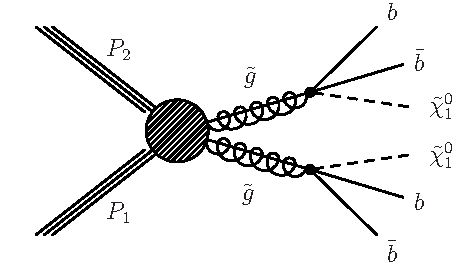
\includegraphics[width=0.45\textwidth]{figures/SusySearches/Ra2b2015/T1bbbb.pdf}
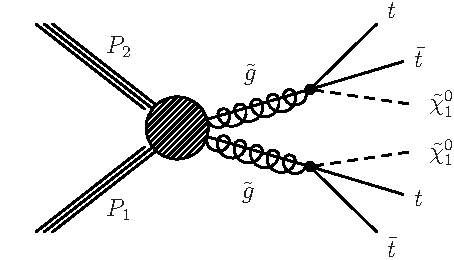
\includegraphics[width=0.45\textwidth]{figures/SusySearches/Ra2b2015/T1tttt.pdf}\\
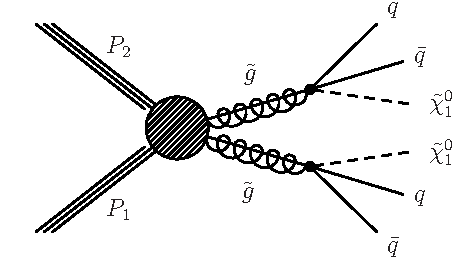
\includegraphics[width=0.45\textwidth]{figures/SusySearches/Ra2b2015/T1qqqq.pdf}
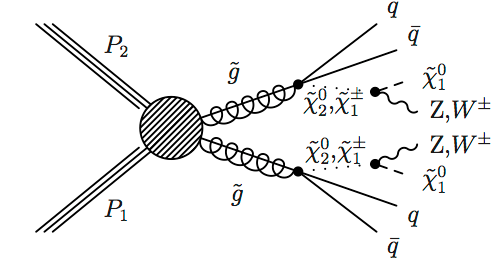
\includegraphics[width=0.45\textwidth]{figures/SusySearches/Ra2b2015/T5vv.pdf}
\caption{
  The simplified models used for the optimization and interpretation of the multi-jet $+$ $\mht$ search. 
  They are T1bbbb (upper left), T1tttt (upper right), T1qqqq (lower left), and T5qqqqVV (lower right) scenarios.
}
\label{fig:Ra2bSMS}
\end{figure}

Events are collected using the hadronic trigger discussed in Section \ref{sec:anatrig}. At level 1 of the trigger system, events are triggered if they have a calorimeter-based $\Ht$ of 175 GeV. If the event is accepted, the
HLT trigger then requires a calorimeter-based $\Ht>$ 280 GeV and a calorimeter-based $\met>$ 70 GeV. Finally, the HLT trigger applies a lower threshold of 350 GeV on the $\Ht$ in coincidence with a threshold on the $\met$ above 100 GeV computed using all particles reconstructed from information from the tracker and calorimeters.

The probability for the trigger to fire on an event that passes the baseline selection is greater than 97\%. The baseline event selection can be summarized as follows. Events are accepted if they have
\begin{itemize}
\item no reconstructed, isolated lepton with a $\pt>10$ GeV and $|\eta|<2.4$, where the isolation is as defined in Equation \ref{eq:isolation};
\item no reconstructed, isolated particle track with a $\pt>10$ GeV and $|\eta|<2.4$;
\item $\Ht>500$ GeV;
\item $\mht>200$ GeV;
\item $\njets\geq$ 4, where jets are required to have a $\pt>30$ GeV and $|\eta|<2.4$, and
\item an azimuthal separation between the $\mht$ and the leading four jets $\Delta\phi(\mht$, jet$_{1,2,3,4})>$ 0.5, 0.5, 0.3, 0.3.
\end{itemize}
After this selection, events are further subdivided into 72 exclusive bins
in a four-dimensional array of $\mht$,
the number of jets,
the number of tagged bottom quark jets,
and $\Ht$. Figure \ref{fig:ra2bArray} shows the boundaries of 6 bins in the $\Ht-\mht$ plane, and 12 bins in the plane of $\njets$$-$$\nbjets$. The 72 bins included in this search are defined by each unique combination of a box in the $\mht$$-$$\Ht$ plane and a box in the $\njets$$-$$\nbjets$ plane. The relative contribution of each~\sm~background in the selected regions is also shown. 
\begin{figure}[h]
\centering
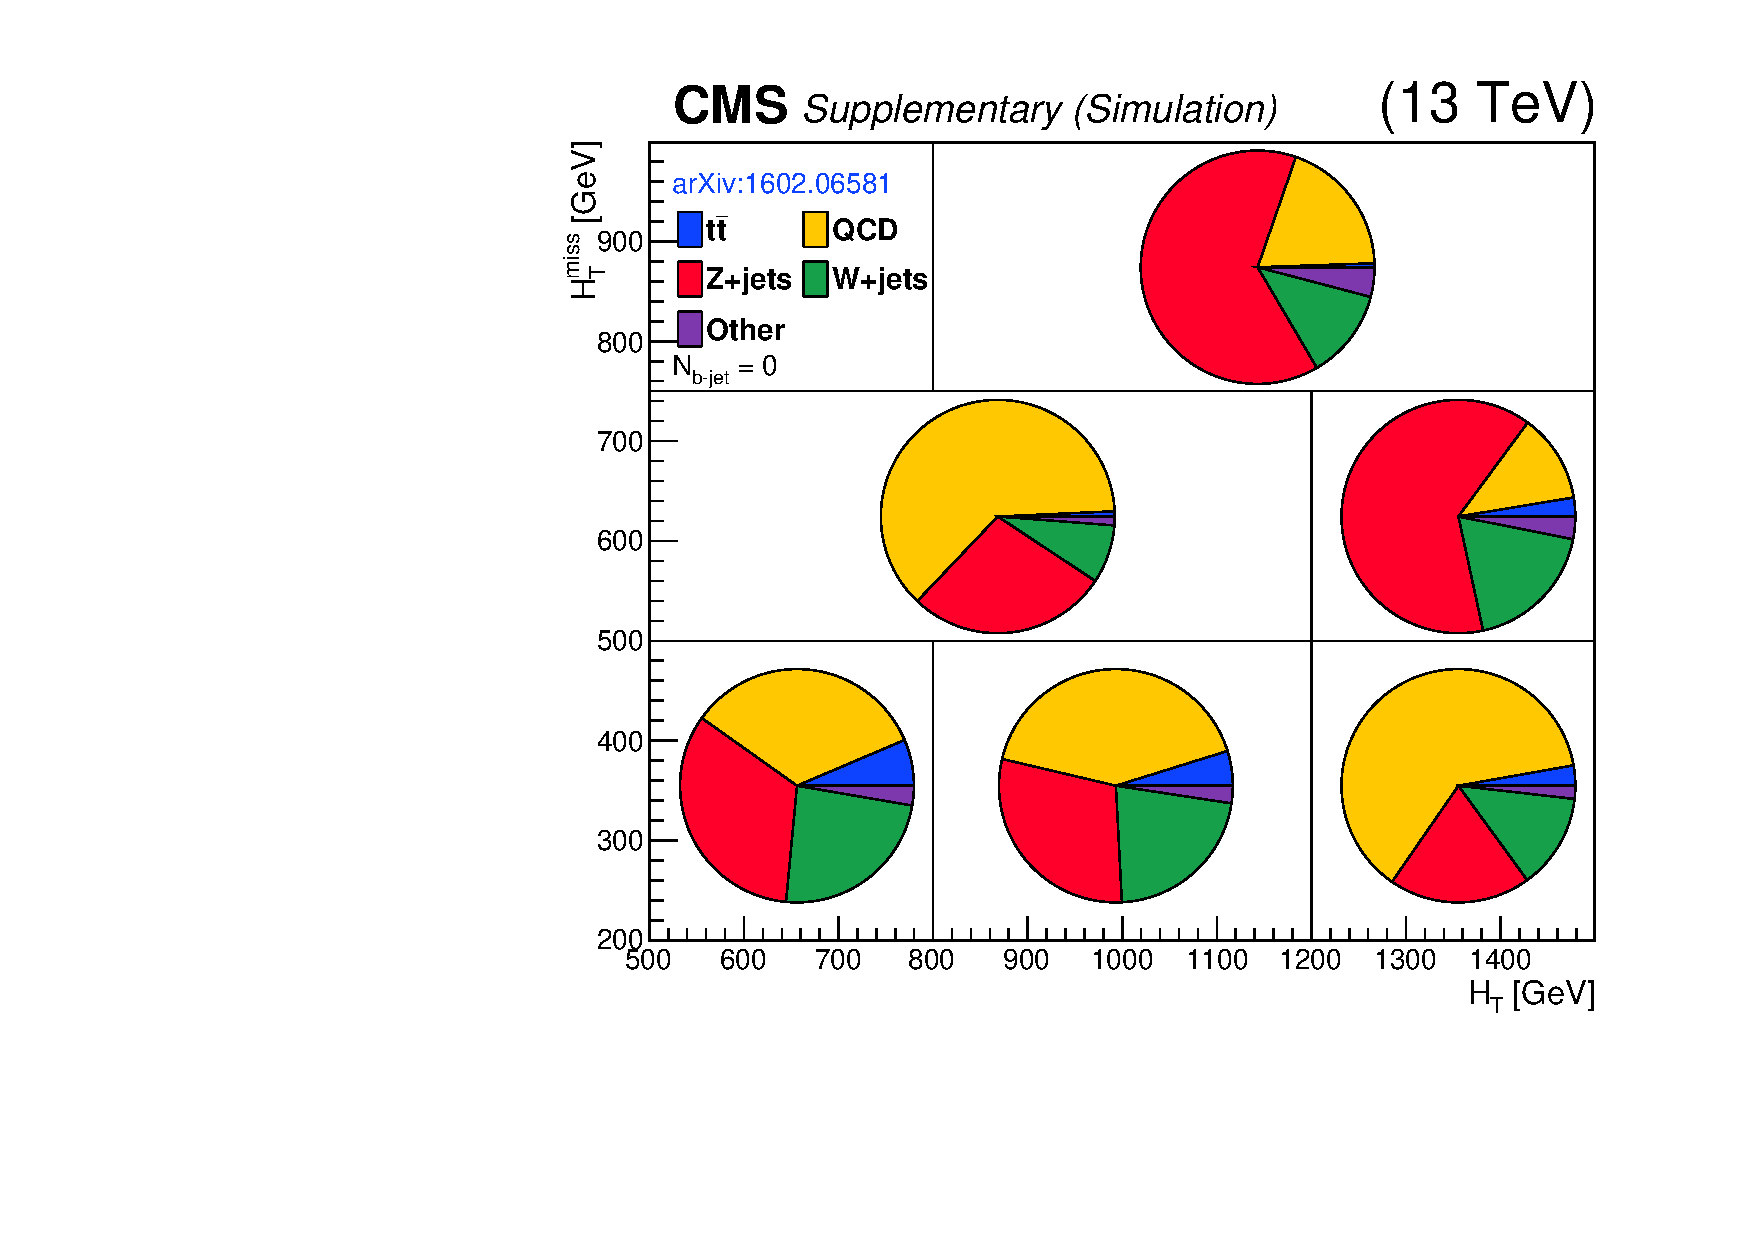
\includegraphics[height=0.442\textwidth]{figures/SusySearches/Ra2b2015/aux/MC_BG_Pie_NB0.pdf}
\hspace{-1cm}
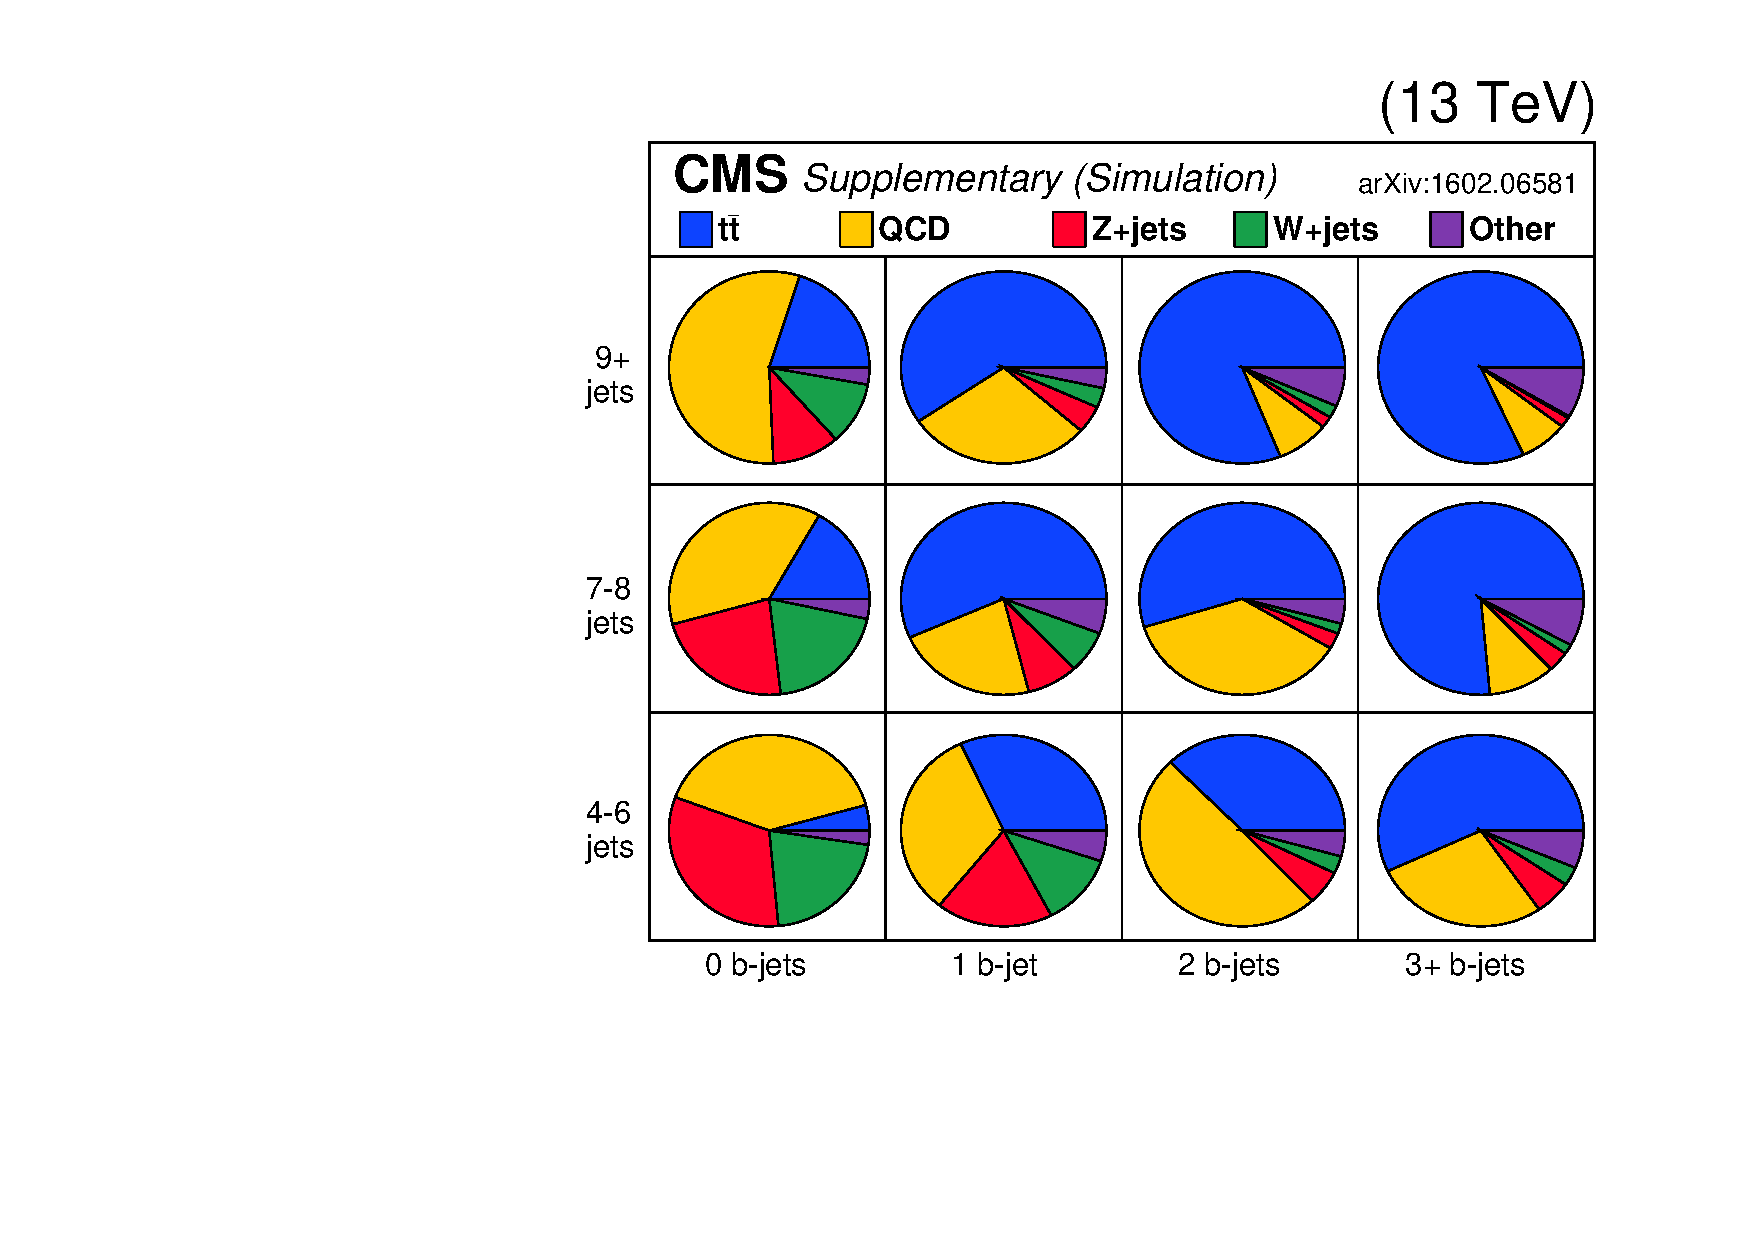
\includegraphics[height=0.445\textwidth]{figures/SusySearches/Ra2b2015/aux/MC_BG_Pie_vs_NJets_NBJets.pdf}
\caption{The signal region boundaries in the planes of $\mht$$-$$\Ht$ (top) and $\njets$$-$$\nbjets$ (bottom) for the multi-jet $+$ $\mht$ 
search. The pie charts represent the relative contributions
 to the~\sm~backgrounds in the region $\njets=$ 4$-$6, $\nbjets=0$ (top), and $\mht=$ 200$-$500 GeV, $\Ht=$ 500$-$750 GeV (bottom).}
\label{fig:ra2bArray}
\end{figure}


\begin{figure}[ht]
\centering
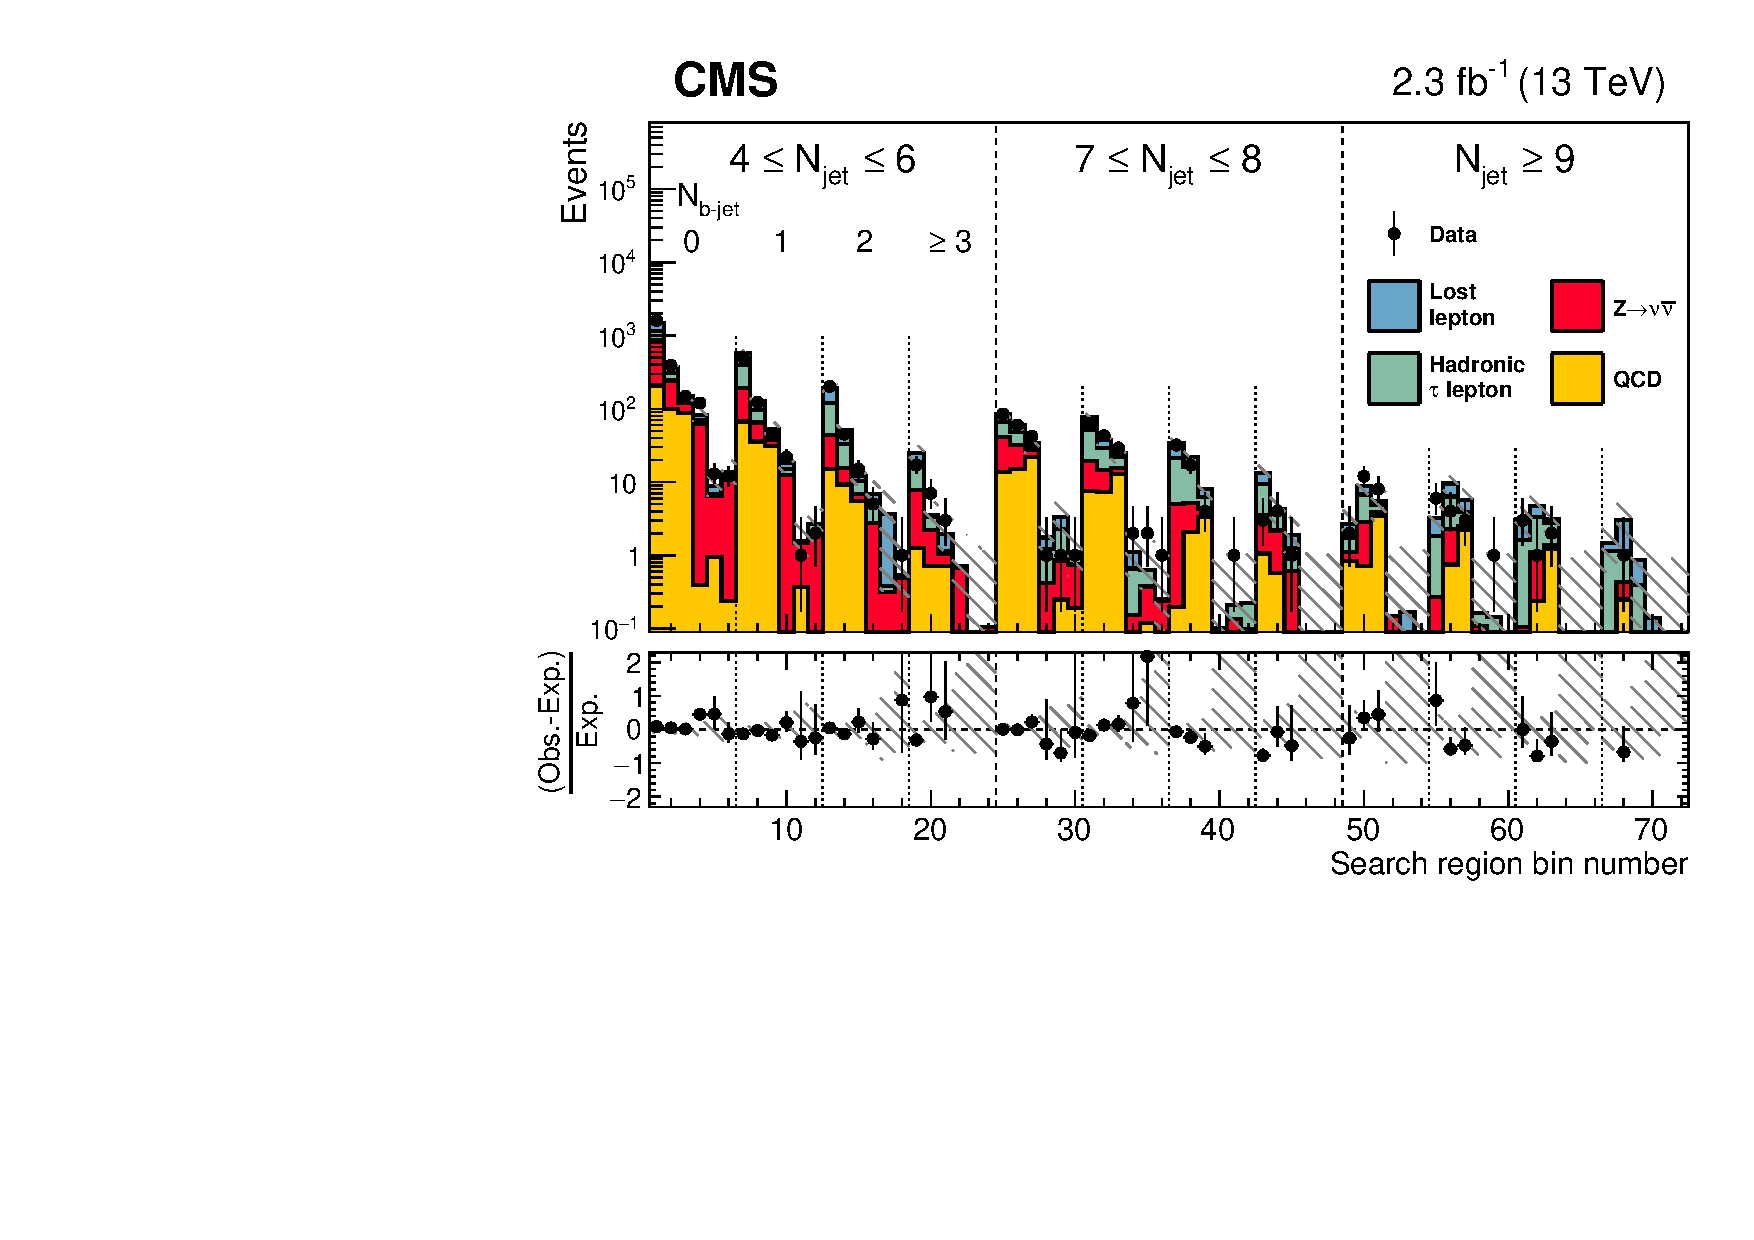
\includegraphics[width=\linewidth]{figures/SusySearches/Ra2b2015/results-plot-prefit.pdf}
\caption{
  Observed numbers of events and corresponding prefit
  SM background predictions
  in the 72 search regions of the analysis,
  with fractional differences shown in the lower panel.
  The shaded regions indicate the total uncertainties in the background
  predictions. For the precise numbering scheme, please see Appendix A of~\cite{Khachatryan:2016kdk}.
}
\label{fig:fit-results}
\end{figure}


The observed numbers of events in the 72 search regions
are shown in Fig.~\ref{fig:fit-results}
in comparison to the summed predictions for the SM backgrounds,
with numerical values tabulated in Appendix A of~\cite{Khachatryan:2016kdk}. The estimation of the QCD background was performed using a data-driven method \cite{Khachatryan:2016kdk} that relates the counts in an inverted $\Delta\phi$ control region to the counts in the signal region. This method is independent from the rebalance and smear method described earlier. 
The comparison between the prediction for the two methods is shown in Fig. \ref{fig:2015CompareQCD}. No evidence of inconsistency is seen between the two independent predictions.
\begin{figure}[ht]
\centering
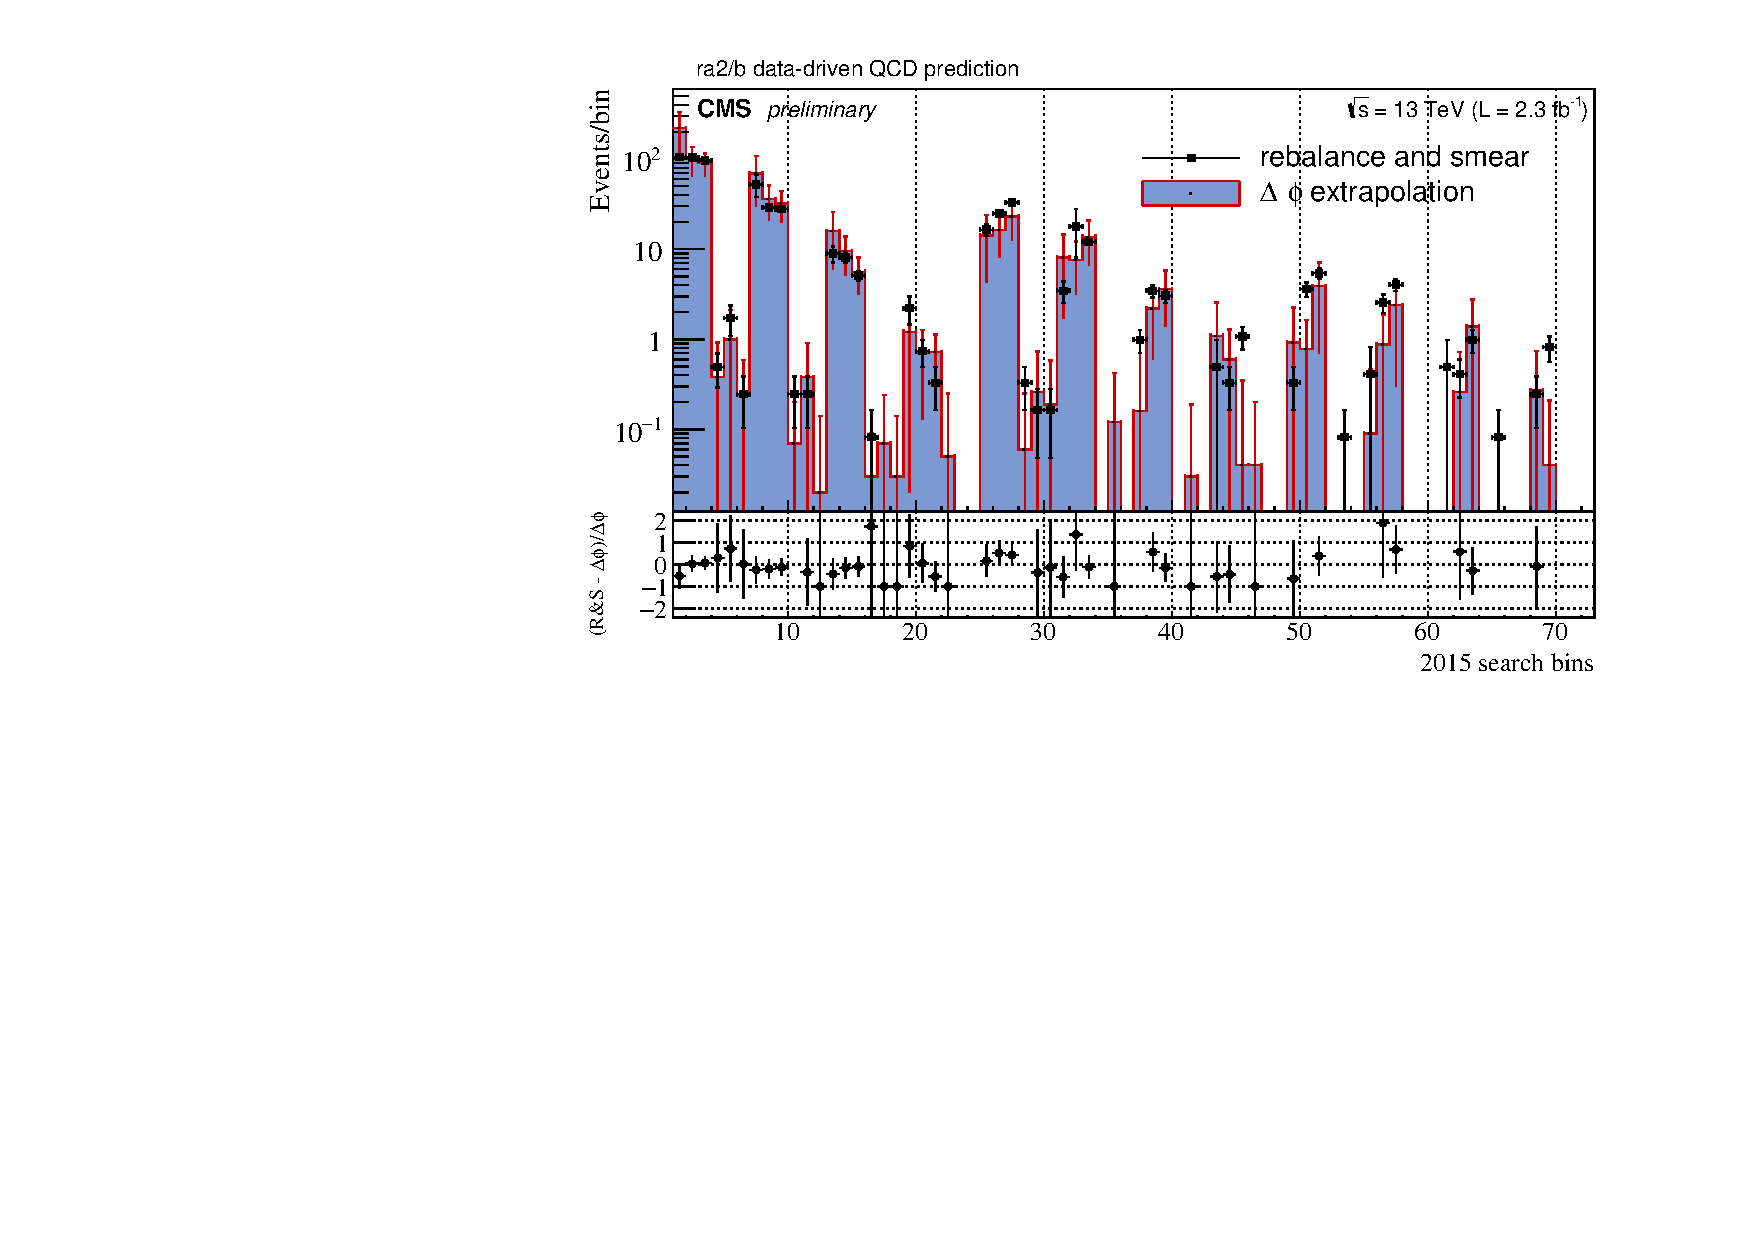
\includegraphics[width=\linewidth]{figures/SusySearches/Ra2b2015/2015CompareQCD.pdf}
\caption{
  The QCD prediction based on the $\Delta\phi$ extrapolation method compared with that of the of rebalance and smear method.}
\label{fig:2015CompareQCD}
\end{figure}
The predicted background is observed to be statistically compatible
with the data for all 72 regions.
Therefore, we do not observe evidence for new physics.
These results are interpreted in the context of the simplified models shown in Fig. \ref{fig:Ra2bSMS}.

For the interpretation, a likelihood fit to data is used to set limits on
the production cross sections of the signal scenarios.
The fitted parameters are the SUSY signal strength,
the yields of the four background classes indicated in Fig.~\ref{fig:fit-results},
and various nuisance parameters.
The limits are determined as a function of $m_{\tilde{\chi}^{0}_{1}}$ and $m_{\tilde{\text{g}}}$.
The likelihood function is the product of Poisson probability functions,
one for each search region,
and constraint terms that account for
uncertainties in the background predictions and signal yields.
These uncertainties are modeled as nuisance parameters
with log-normal probability density functions.
Correlations are taken into account where appropriate.
The signal model uncertainties associated with
the renormalization and factorization scales, ISR,
the jet energy scale,
the b-jet tagging,
and the statistical fluctuations
vary substantially with the event kinematics
and are evaluated as a function of $m_{\tilde{\chi^{0}_{1}}}$ and $m_{\tilde{\text{g}}}$.
The test statistic is
$q_\mu =  - 2 \ln \left( \mathcal{L}_\mu/\mathcal{L}_\text{max} \right)$,
where $\mathcal{L}_\text{max}$ is the maximum likelihood
determined by allowing all parameters including the profile likelihood for the
SUSY signal strength $\mu$ to vary,
and $\mathcal{L}_\mu$ is the maximum likelihood for a fixed signal strength.
To set limits,
we use asymptotic results for the test statistic~\cite{Cowan:2010js}
and the CL$_\mathrm{s}$
method described in Refs.~\cite{Junk1999,bib-cls}. 
Uncertainties in the signal modeling are taken into account when the limits are determined: simulation sample size, luminosity determination ($4.6\%$), lepton and isolated track veto, b-tag efficiency corrections used to scale simulation to data, trigger efficiency, QCD renormalisation and factorization scales, initial/final state radiation (ISR/FSR), signal acceptance and efficiency arising from the jet energy-momentum corrections, jet energy-momentum resolutions, and propagated to \MET, parton distribution functions (PDF) of the proton. More details are provided in Refs.~\cite{cms-note-2011-005,Khachatryan:2015vra}.

\begin{figure*}[htbp]
\centering
    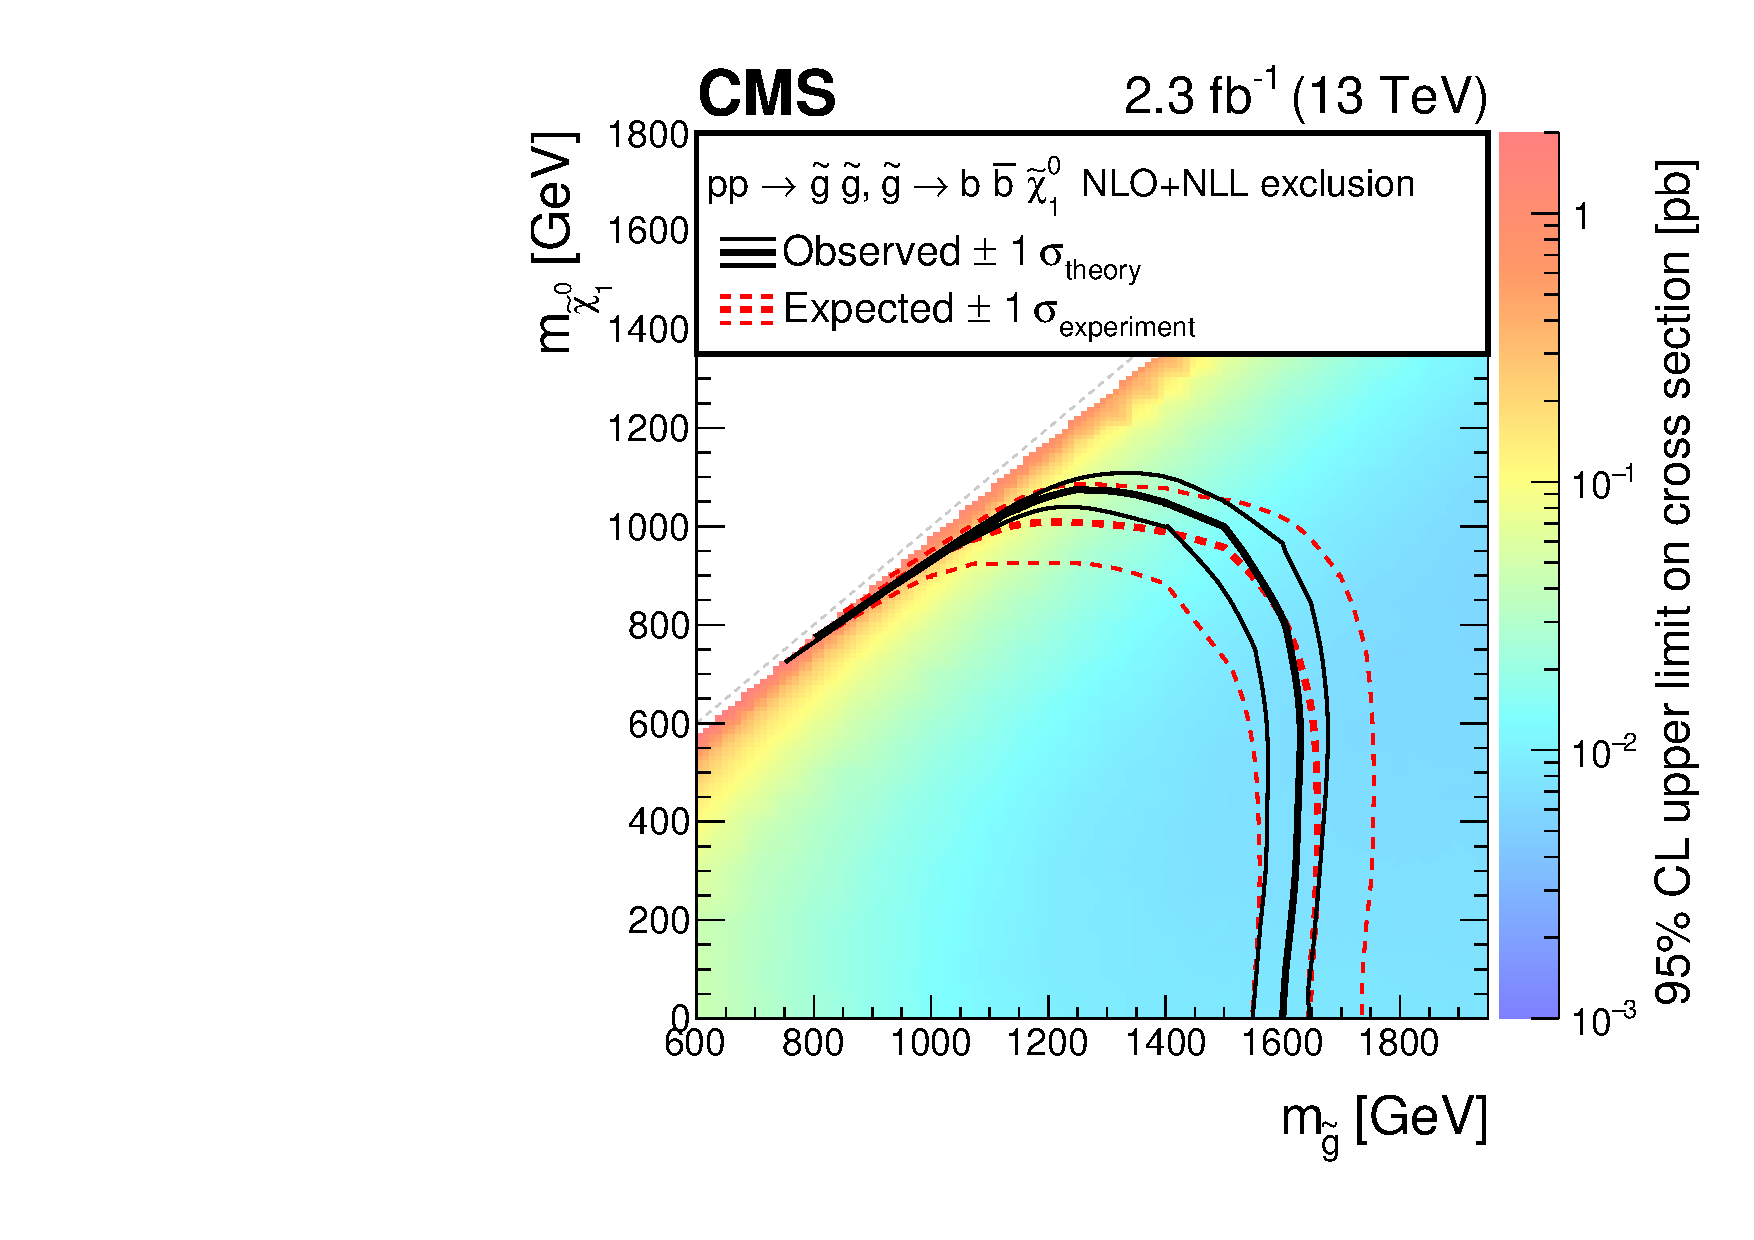
\includegraphics[width=0.48\textwidth]{figures/SusySearches/Ra2b2015/SMSbbbbXSEC.pdf}
    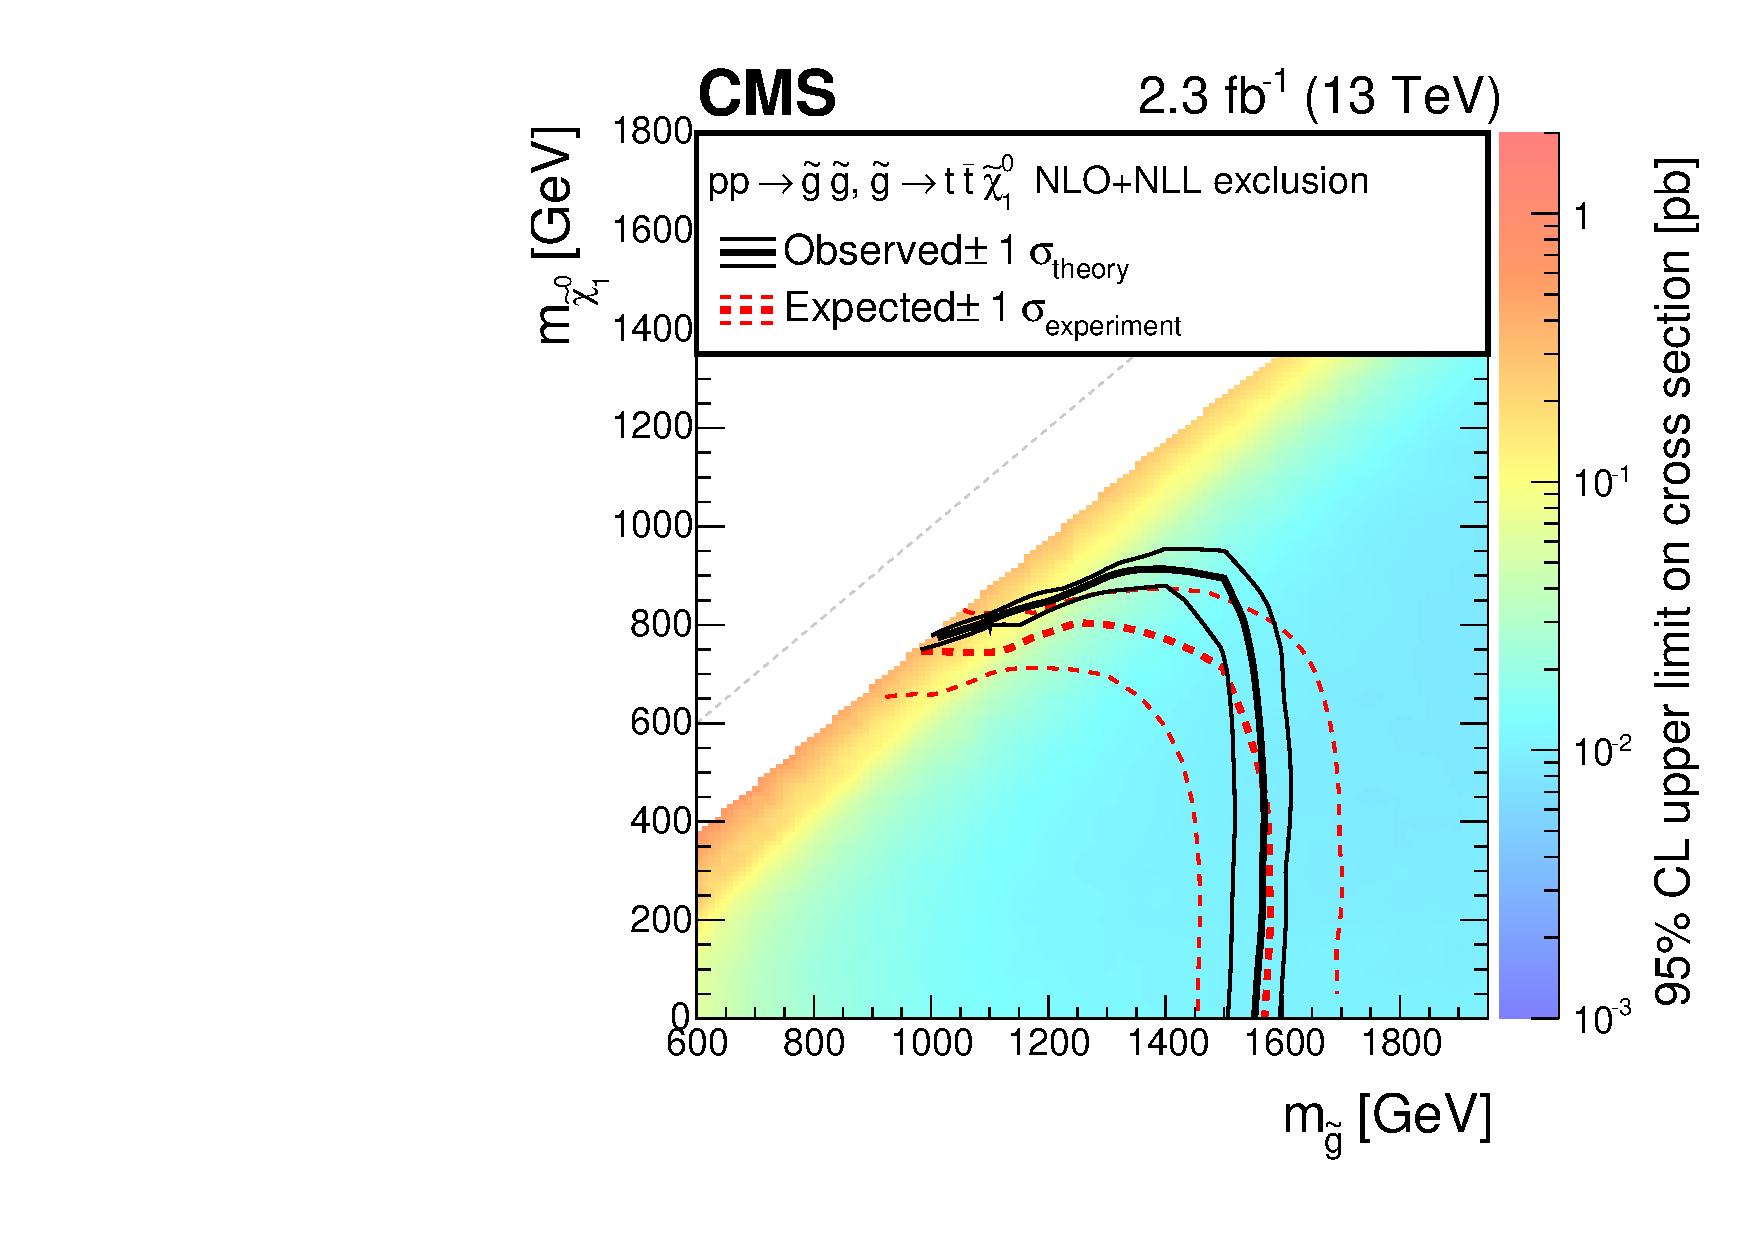
\includegraphics[width=0.48\textwidth]{figures/SusySearches/Ra2b2015/SMSttttXSEC.pdf} \\
    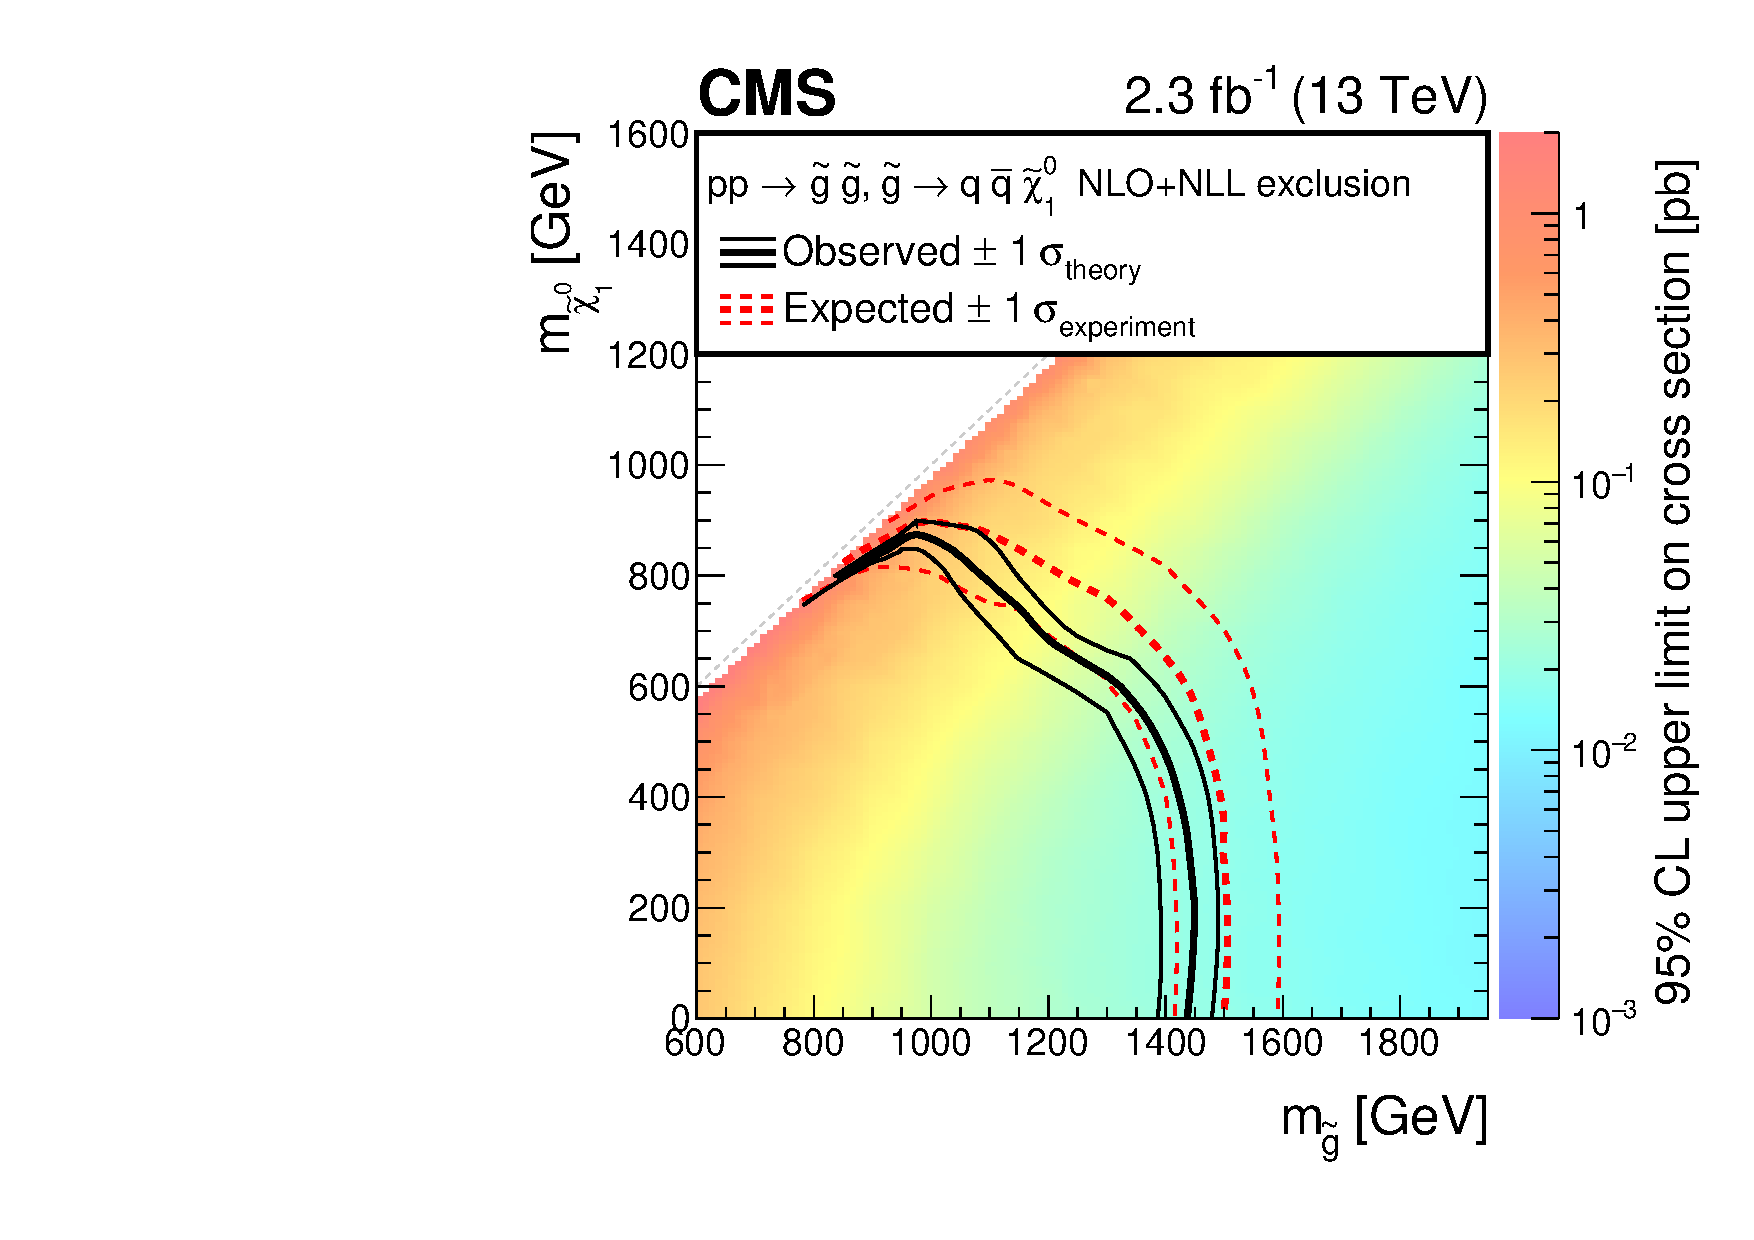
\includegraphics[width=0.48\textwidth]{figures/SusySearches/Ra2b2015/SMSqqqqXSEC.pdf}
    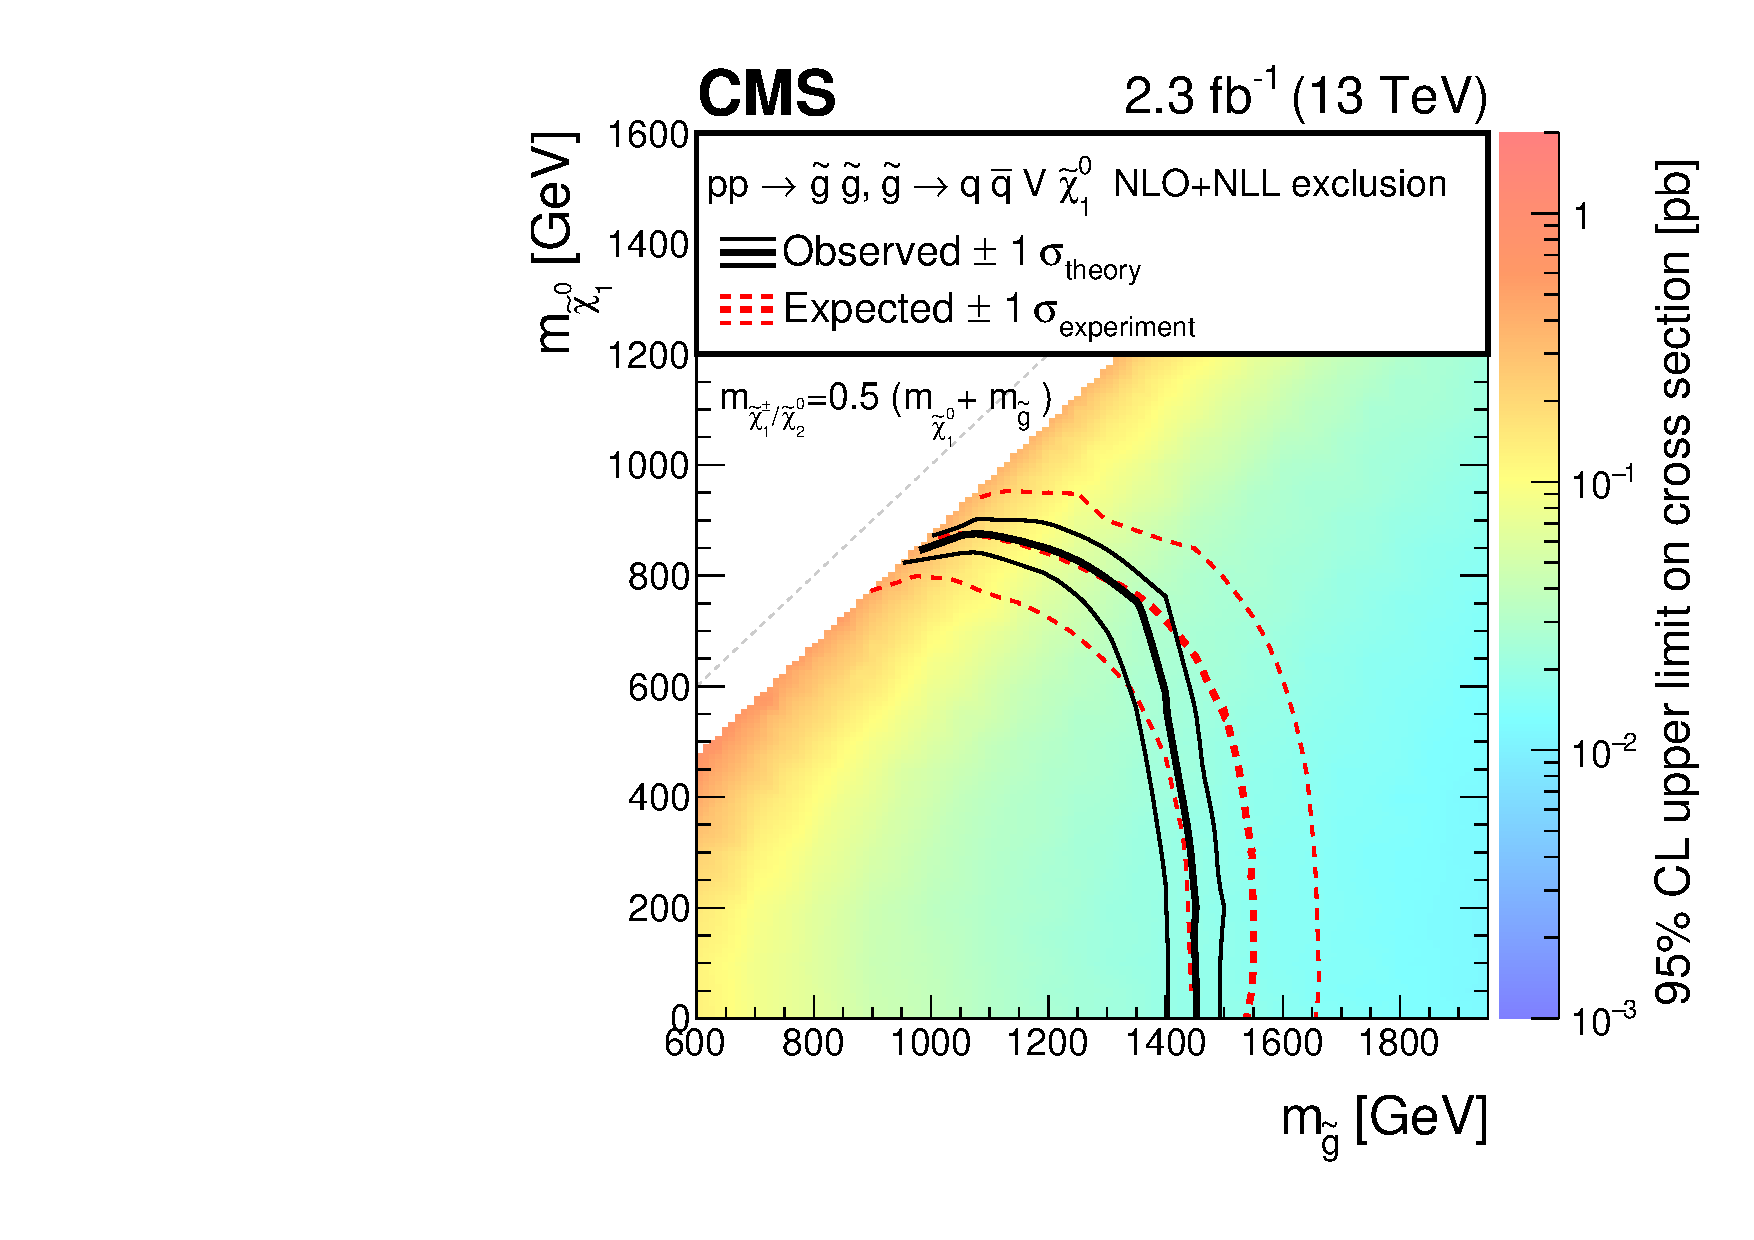
\includegraphics[width=0.48\textwidth]{figures/SusySearches/Ra2b2015/SMSqqqqVVXSEC.pdf}
    \caption{
      The 95\% CL upper limits on the production
      cross sections for the T1bbbb (upper left),
      T1tttt (upper right), T1qqqq (lower left),
      and T5qqqqVV (lower right) simplified models of supersymmetry,
      shown as a function of the gluino and LSP masses $m_{\tilde{\text{g}}}$ and $\tilde{\chi}^{0}_{1}$.
      For the T5qqqqVV model,
      the masses of the intermediate $\tilde{\chi}^{0}_{2}$ and $\tilde{\chi}^{\pm}_{1}$  states
      are taken to be the mean of $m_{\tilde{\chi}^{0}_{1}}$ and $m_{\tilde{\text{g}}}$.
      The solid (black) curves show the observed exclusion contours
      assuming the NLO+NLL cross
      sections, with the corresponding $\pm$1~standard
      deviation uncertainties~\cite{Borschensky:2014cia}.
      The dashed (red) curves are the expected limits
      with $\pm$1 standard deviation experimental uncertainties.
      The dashed (grey) lines indicate the $\tilde{\chi}^{0}_{1}=m_{\tilde{\text{g}}}$ diagonal.
    }
    \label{fig:limits}
\end{figure*}

We proceed to evaluate 95\% confidence level (CL) upper limits
on the signal cross sections.
The NLO+NLL cross section is used as a reference
to evaluate corresponding 95\% CL exclusion curves.
In addition to the observed limits,
expected limits are derived by evaluating the
expected Poisson fluctuations around the predicted
numbers of background events when evaluating the test statistic.
The potential contributions of signal events to the control regions
are taken into account.
Specifically,
the number of events in each CR is corrected
to include the predicted number of signal events,
in the context of the model being examined,
to derive the total effective number of background events
expected in each search region.
This total effective background is used when determining the limits.

The results are shown in Fig.~\ref{fig:limits}. 
For a massless LSP,
we exclude gluinos with masses below 1600, 1550, 1440, and 1450~\GeV,
respectively,
for the T1bbbb, T1tttt, T1qqqq, and T5qqqqVV scenarios. The observed exclusion curves are also shown for the cases in which the signal cross section is varied by changing the renormalization and factorization scales by a factor of 2 and using the PDF4LHC recommendation~\cite{Botje:2011sn} for the PDF uncertainty to illustrate the sensitivity of the exclusion to the signal cross section uncertainty.
These results significantly extend those that were
obtained at $\sqrt{s}=8~\TeV~$,
for which the corresponding limits are around
1150~\GeV~\cite{Chatrchyan:2013wxa,Chatrchyan:2014lfa} for the
three T1 models and 1280~\GeV~\cite{Chatrchyan:2014lfa} for the T5 model.
